% Supplementary material for "Walls or cascade?" (main.tex).
%
% Build: make (in this directory), which builds both documents: each reads the
% other's labels through xr-hyper, as S-<label> in main.tex and M-<label> here.
% Every number below that comes from a run is printed by numbers.py, which also
% writes tab_protocol.tex, tab_verify.tex and tab_layers.tex; the figures are made
% by `make figs`.
\documentclass[aip,pop,reprint,amsmath,amssymb,superscriptaddress,floatfix]{revtex4-2}

\usepackage[utf8]{inputenc}
\usepackage[T1]{fontenc}
\usepackage{graphicx}
\usepackage{bm}
\usepackage{xr-hyper}
\usepackage[hidelinks]{hyperref}
\graphicspath{{../../results/P_tg_mhd/fig/}}

\newcommand{\Rey}{\mathrm{Re}}
\newcommand{\vv}{\bm{v}}
\newcommand{\BB}{\bm{B}}
\newcommand{\eps}{\varepsilon}
% after the macros: the other document's labels carry captions that use them
\externaldocument[M-]{main}

\begin{document}

\title{Supplementary material for ``Walls or cascade? A pre-registered test of wall
dissipation in decaying magnetohydrodynamic turbulence''}

\author{Alessandro De Rosis}
\email{alessandro.derosis@manchester.ac.uk}
\affiliation{The University of Manchester, Manchester M13 9PL, United Kingdom}

\date{\today}

\maketitle

\renewcommand{\thesection}{S\arabic{section}}
\renewcommand{\thetable}{S\arabic{table}}
\renewcommand{\thefigure}{S\arabic{figure}}
\renewcommand{\theequation}{S\arabic{equation}}

Equations, sections, figures and tables numbered without an S are those of the
paper. Every number below that comes from a run is printed, with its source, by the
script that produces the paper's numbers (\texttt{paper/tg\_mhd/numbers.py} in the
repository).

%===============================================================================
\section{Verification of the method}
\label{s:method}
%===============================================================================

\emph{The parity wall.} Three tests in the repository check Eq.~(\ref{M-eq:parity})
(\texttt{validation/mhd\_parity\_wall.cpp}). First, with free slip and either parity,
the box of $N$ nodes reproduces the periodic $2\pi$ box of $2(N-1)$ nodes to
$10^{-14}$, node for node and transient included. Second, $\BB\cdot\bm{n}$ on the wall
nodes stays at $10^{-32}$. Third, in the no-slip box the exact decay of the
conducting-wall eigenmode $\BB=B_0(\sin x\cos y,-\cos x\sin y,0)$, which leaves the
fluid at rest, converges at second order (order $2.00$ over $N=17$, $33$, $65$).

\emph{The two implementations.} The C++20/Kokkos code and the CUDA code share no
source. Their host builds agree to every printed digit over 815 steps at $N=65$,
$\Rey=200$, with free and no slip, and the CUDA build on the device agrees with the
Kokkos reference to within $5.5\times10^{-16}$ of each diagnostic's scale, in four
verification jobs, each with free and no slip. The runs behind the paper's numbers
took $34.1$ GPU-hours: the ladder, its two controls, and a second round with the top
rung, the insulating pair, and reruns of the lower rungs that also write the viscous
and Ohmic parts of the profile. The reruns that wrote the fields of
Sec.~\ref{M-sec:fields} took $1.5$ more, and the first ladder, run with the estimator
of Sec.~\ref{s:estimator}, $8.2$.

\emph{Run C2 of Pouquet et al.} The free-slip box A at $\Rey=1000$ is run C2 of
Ref.~\onlinecite{pouquet2010}. Its minimum ratio of magnetic to kinetic energy is
$E_M/E_V=0.3695$ and $0.3693$ at $N=384$ and $512$, reached at $t=7.3$, against their
$0.35$, and the first maximum of $\Omega_M/\Omega_V$ after its initial fall is $2.154$
and $2.159$, against their ``2.''. Our ratio is converged to four figures between the
two grids and lies $5.5$\% above theirs, which is quoted to two figures.

We attribute the gap to the resolution of C2. It is the coarsest run of
Ref.~\onlinecite{pouquet2010}: pseudo-spectral on an equivalent grid of $128^3$ over
the period $2\pi$, i.e.\ $64$ points across our box. Its Table~1 lists
$\delta k_{\max}=0.8$, where $\delta$ is the logarithmic decrement of a fit
$E_T(k)\propto k^{-n}e^{-2\delta k}$ to the energy spectrum and $k_{\max}=N/3$. That is
below $\delta k_{\max}\approx1$, at which the authors stop an ideal computation, and
below the $\delta k_{\max}\ge2$ by which they call their $2048^3$ runs well resolved;
their other two $128^3$ runs have $1.9$ and $2.1$, and C2 has no companion at higher
resolution. Under-resolution moves our own ratio the same way: $0.357$ at $N=97$,
reached at $t=9.8$, and $0.329$ at $N=65$, still falling at $t=10$. The two codes
under-resolve by different mechanisms, so the common direction is suggestive rather
than conclusive.

%===============================================================================
\section{The record of the protocol}
\label{s:protocol}
%===============================================================================

The two outcomes of Sec.~\ref{M-sec:intro} were stated, qualitatively, on 25 September
2026 in a plan that is not in the repository, and nothing there dates them. The rules
of Sec.~\ref{M-sec:protocol} were committed with the job scripts. A commit's date is
written by its author, so Table~\ref{stab:protocol} also gives the time at which each
commit reached GitHub, from GitHub's server-side record of the pushes to the
repository. A copy of that record, as GitHub's public interface returned it on
2 October 2026, is kept in the repository (\texttt{paper/tg\_mhd/provenance/}) with
the request that fetched it; GitHub returns it to anyone for about three months after
a push. Each rule was on GitHub within $80$\,s of being committed. The estimator was
corrected after the first ladder had failed its gate (Sec.~\ref{s:estimator}); the
observable it estimates and the gate did not change. The Mach control, and the
decision rule and the precision control for the top rung, were fixed after the lower
rungs had been run, and seen, and before the runs they judge. Before 30 September the ladder's script asked
only that B$-$A exceed its band and trend monotonically over at least three rungs;
the decision rule of Sec.~\ref{M-sec:protocol}, which is the one applied in the
paper, replaced that with a test at the top rung, fixed with the job script that ran
it.
% TODO(author): add the cluster's accounting of when each job was submitted (sacct;
% provenance/README.md says how), which closes the other end of each interval.

\begin{table*}
\caption{\label{stab:protocol}When each rule was fixed: the commit, its time by the
author's clock, and the time at which it reached GitHub by GitHub's push record, on
the same day. All times UTC, 2026.}
\begin{ruledtabular}
\begin{tabular}{lcccc}
rule & commit & committed (UTC) & pushed (UTC) & lag (s) \\
\hline
observable, peak rule, gate & \texttt{663929c} & 27 Sep, 11:57:38 & 11:58:24 & 46 \\
estimator of $f_m$ corrected & \texttt{9f65706} & 28 Sep, 11:55:32 & 11:56:52 & 80 \\
Mach control & \texttt{cd07f45} & 29 Sep, 06:22:12 & 06:22:15 & 3 \\
decision rule, FP64 control ($\Rey=2000$) & \texttt{d061ee8} & 30 Sep, 20:03:29 & 20:03:34 & 5 \\
the budget test, $\phi$ & \texttt{8376e66} & 02 Oct, 12:00:24 & 12:00:26 & 2 \\
the four controls & \texttt{f7f55ba} & 03 Oct, 04:19:57 & 04:19:59 & 2 \\
\end{tabular}

\end{ruledtabular}
\end{table*}

%===============================================================================
\section{The estimator of the wall share}
\label{s:estimator}
%===============================================================================

Counting whole node layers, every node with $kh<m\delta$, measures a layer of
thickness $(\lceil m\delta/h\rceil-\tfrac12)h$ rather than $m\delta$, because the
nodes with $d=kh$ fill exactly the slab between $(k-\tfrac12)h$ and $(k+\tfrac12)h$
(Sec.~\ref{M-sec:method}): $0.91\delta$ at $N=384$ and $1.07\delta$ at $N=512$ for
$\Rey=1000$. Our first ladder counted layers. At every rung of every box with a
turbulent peak, eight in all, it failed the gate: the worst of $f_1$, $f_2$ and $f_4$
differed between the two grids by $6.5$--$24.6$\%, while $\eps$ at the peak agreed to
$1$\%. Moved to the exact band, by interpolating each grid's three samples, the same
series pass, the worst difference becoming $2.9$\%. Swept across $N=33$ to $49$ at fixed physics ($\Rey=100$), the count makes
$f_4$ jump between $0.52$ and $0.60$ each time $4\delta/h$ crosses a node, while
Eq.~(\ref{M-eq:within}) keeps it within $0.561$--$0.566$. Any layer, shell or
threshold observable on a lattice can do this.

%===============================================================================
\section{Resolution gate and controls}
\label{s:gate}
%===============================================================================

Table~\ref{stab:verify} gives the resolution gate and the controls of
Sec.~\ref{M-sec:verify} rung by rung.

\begin{table*}
\caption{\label{stab:verify}Resolution gate and controls. Relative differences of
$f_1$, $f_2$ and $f_4$ at the turbulent peak between the two grids of each rung, the
band of B$-$A (the two grid differences of $f_1$, added), and the shift of B$-$A in
the control run: Mach, $u_0$ halved; FP64, double precision at $N=512$.}
\begin{ruledtabular}
\begin{tabular}{rccccl}
$\mathrm{Re}$ & $N$ & A: $\Delta f_1/\Delta f_2/\Delta f_4$ (\%) & B: $\Delta f_1/\Delta f_2/\Delta f_4$ (\%) & band & control shift \\
\hline
250 & 192, 256 & 0.7/0.2/0.1 & 1.0/0.7/0.2 & 0.0020 & -- \\
500 & 256, 384 & 0.8/0.5/1.0 & 2.1/1.5/0.7 & 0.0030 & Mach, $-0.0014$ \\
1000 & 384, 512 & 0.7/0.7/0.3 & 0.2/0.1/0.2 & 0.0004 & Mach, $<10^{-4}$ \\
2000 & 512, 640 & 3.0/1.3/0.8 & 0.5/0.4/0.3 & 0.0021 & FP64, $<10^{-4}$ \\
\end{tabular}

\end{ruledtabular}
\end{table*}

%===============================================================================
\section{The thickness of the layer}
\label{s:layers}
%===============================================================================

Table~\ref{stab:layers} repeats the readings of Table~\ref{M-tab:windows} for the
layers $2\delta$ and $4\delta$ thick. The bands are the two grid differences of each
layer's share, added, as for $\delta$; the largest is $0.0056$ at the peak and
$0.0016$ over a time window. The thicker layers read as the thinnest does. B$-$A is
positive in every reading at every rung, from $0.019$ to $0.115$. From $\Rey=250$ to
$2000$ it changes by $+2$\% within $2\delta$ and $-20$\% within $4\delta$ over
$t=2$--$6$, against $-3$\% within $\delta$; falls by $12$--$42$\% and $23$--$35$\%
over the windows that reach further into the decay, against $18$--$43$\%; and falls by
$68$\% and $67$\% at the peak, against $51$\%.

\begin{table*}
\caption{\label{stab:layers}B$-$A in the share of the dissipation within $m\delta$
of the walls, at the turbulent peak and integrated over the time windows of
Table~\ref{M-tab:windows}, on the finer grid of each rung. The last column is the
change from $\Rey=250$ to $2000$.}
\begin{ruledtabular}
\begin{tabular}{lcccccc}
reading & $m$ & 250 & 500 & 1000 & 2000 & change (\%) \\
\hline
at the peak (pre-registered) & 1 & 0.073 & 0.065 & 0.063 & 0.036 & $-51$ \\
 & 2 & 0.075 & 0.076 & 0.065 & 0.024 & $-68$ \\
 & 4 & 0.058 & 0.050 & 0.064 & 0.019 & $-67$ \\
integrated, $t=2$--$6$ & 1 & 0.049 & 0.048 & 0.051 & 0.048 & $-3$ \\
 & 2 & 0.047 & 0.044 & 0.051 & 0.048 & $+2$ \\
 & 4 & 0.060 & 0.049 & 0.050 & 0.048 & $-20$ \\
integrated, $t=2$--$10$ & 1 & 0.059 & 0.055 & 0.054 & 0.048 & $-18$ \\
 & 2 & 0.055 & 0.056 & 0.057 & 0.048 & $-12$ \\
 & 4 & 0.063 & 0.061 & 0.059 & 0.049 & $-23$ \\
integrated, $t=3$--$10$ & 1 & 0.066 & 0.059 & 0.055 & 0.046 & $-29$ \\
 & 2 & 0.066 & 0.062 & 0.058 & 0.044 & $-34$ \\
 & 4 & 0.066 & 0.070 & 0.063 & 0.044 & $-32$ \\
integrated, $t=4$--$10$ & 1 & 0.082 & 0.072 & 0.064 & 0.050 & $-39$ \\
 & 2 & 0.084 & 0.080 & 0.070 & 0.049 & $-42$ \\
 & 4 & 0.078 & 0.088 & 0.077 & 0.050 & $-35$ \\
integrated, $t=5$--$10$ & 1 & 0.095 & 0.085 & 0.072 & 0.054 & $-43$ \\
 & 2 & 0.093 & 0.100 & 0.084 & 0.056 & $-40$ \\
 & 4 & 0.087 & 0.115 & 0.098 & 0.061 & $-30$ \\
\end{tabular}

\end{ruledtabular}
\end{table*}

%===============================================================================
\section{Insulating walls}
\label{s:insul}
%===============================================================================

The pair A$'$, B$'$ was meant to show whether the result needs a conducting wall. It
cannot. A$'$ passes the gate (worst $0.8$\%), and $88$\% of the dissipation within
$\delta$ of its walls is Ohmic ($F_1=0.31$ and $0.27$ at $\Rey=500$ and $1000$). B$'$
has no turbulent peak by $t=10$ at either $\Rey$. It puts more of its dissipation
within $\delta$ of the walls than any other box, $F_1=0.63$ and $0.69$, and these
agree between its two grids to $1.4$\% and $1.7$\%. So B$'-$A$'$ ($+0.32$ and $+0.42$
over $t=2$--$10$) compares a box that has not become turbulent with one that has, and
under a different initial field from B$-$A.

B$'$ is also the only box in which the field crosses a no-slip wall, the
configuration of a Hartmann layer.\cite{sommeria1982,knaepen2008} With the field
normal to the wall, $B_n$, and a tangential velocity $U$ outside the layer, the
tangential momentum and induction equations in the layer are, in Alfv\'en units,
$\nu u''+B_nb'=0$ and $B_nu'+\eta b''=0$, primes denoting derivatives along the
normal. They give $u=U(1-e^{-z/\delta_H})$ with $\delta_H=\sqrt{\nu\eta}/|B_n|$, and a
dissipation per unit area of
\begin{equation}
  \int_0^\infty\!\left(\nu u'^2+\eta b'^2\right)dz = U^2|B_n|\sqrt{\nu/\eta},
  \label{seq:hartmann}
\end{equation}
half of it viscous and half Ohmic. At $\mathrm{Pm}=1$, $\delta_H=1/(\Rey|B_n|)$ has
the scaling of Kato's layer, and Eq.~(\ref{seq:hartmann}) does not depend on
$\Rey$. The field $\BB_I$ of Eq.~(\ref{M-eq:bi}) is normal to every face at $t=0$, with
$|B_n|$ up to $2b_0=1.15$ on the two faces normal to $z$ and up to $b_0$ on the other
four. There a Hartmann layer would be $0.14h$ and $0.28h$ thick at $\Rey=1000$, and
$0.21h$ and $0.42h$ at $\Rey=500$, on the finer grids. These are estimates from the
initial field: we have not measured the layers of B$'$, and its integrated share
agrees between grids that could not resolve them. We draw no conclusion from B$'$ or
from B$'-$A$'$.

%===============================================================================
\section{The fields at a later time}
\label{s:fields46}
%===============================================================================

Figures~\ref{sfig:snap46} and~\ref{sfig:vol46} repeat Figs.~\ref{M-fig:snap23}
and~\ref{M-fig:vol23} at $t=4.6$, by the later maxima of the dissipation. By then the
bulk of both MHD boxes is more finely structured and A's near-wall plane has
quietened, but the contrast of Sec.~\ref{M-sec:fields} remains: in the plane
$0.58\delta$ above the bottom wall, B's viscous dissipation is $6.8$ times A's and its
Ohmic $0.68$ of A's. In three dimensions both MHD boxes have broken up into finer
sheets, and the viscous dissipation of the no-slip box forms ring-like patterns on
its faces. The box without a field dissipates $3.3$ times its box mean in its
near-wall plane, about $3.2$ times B's relative level.

\begin{figure*}
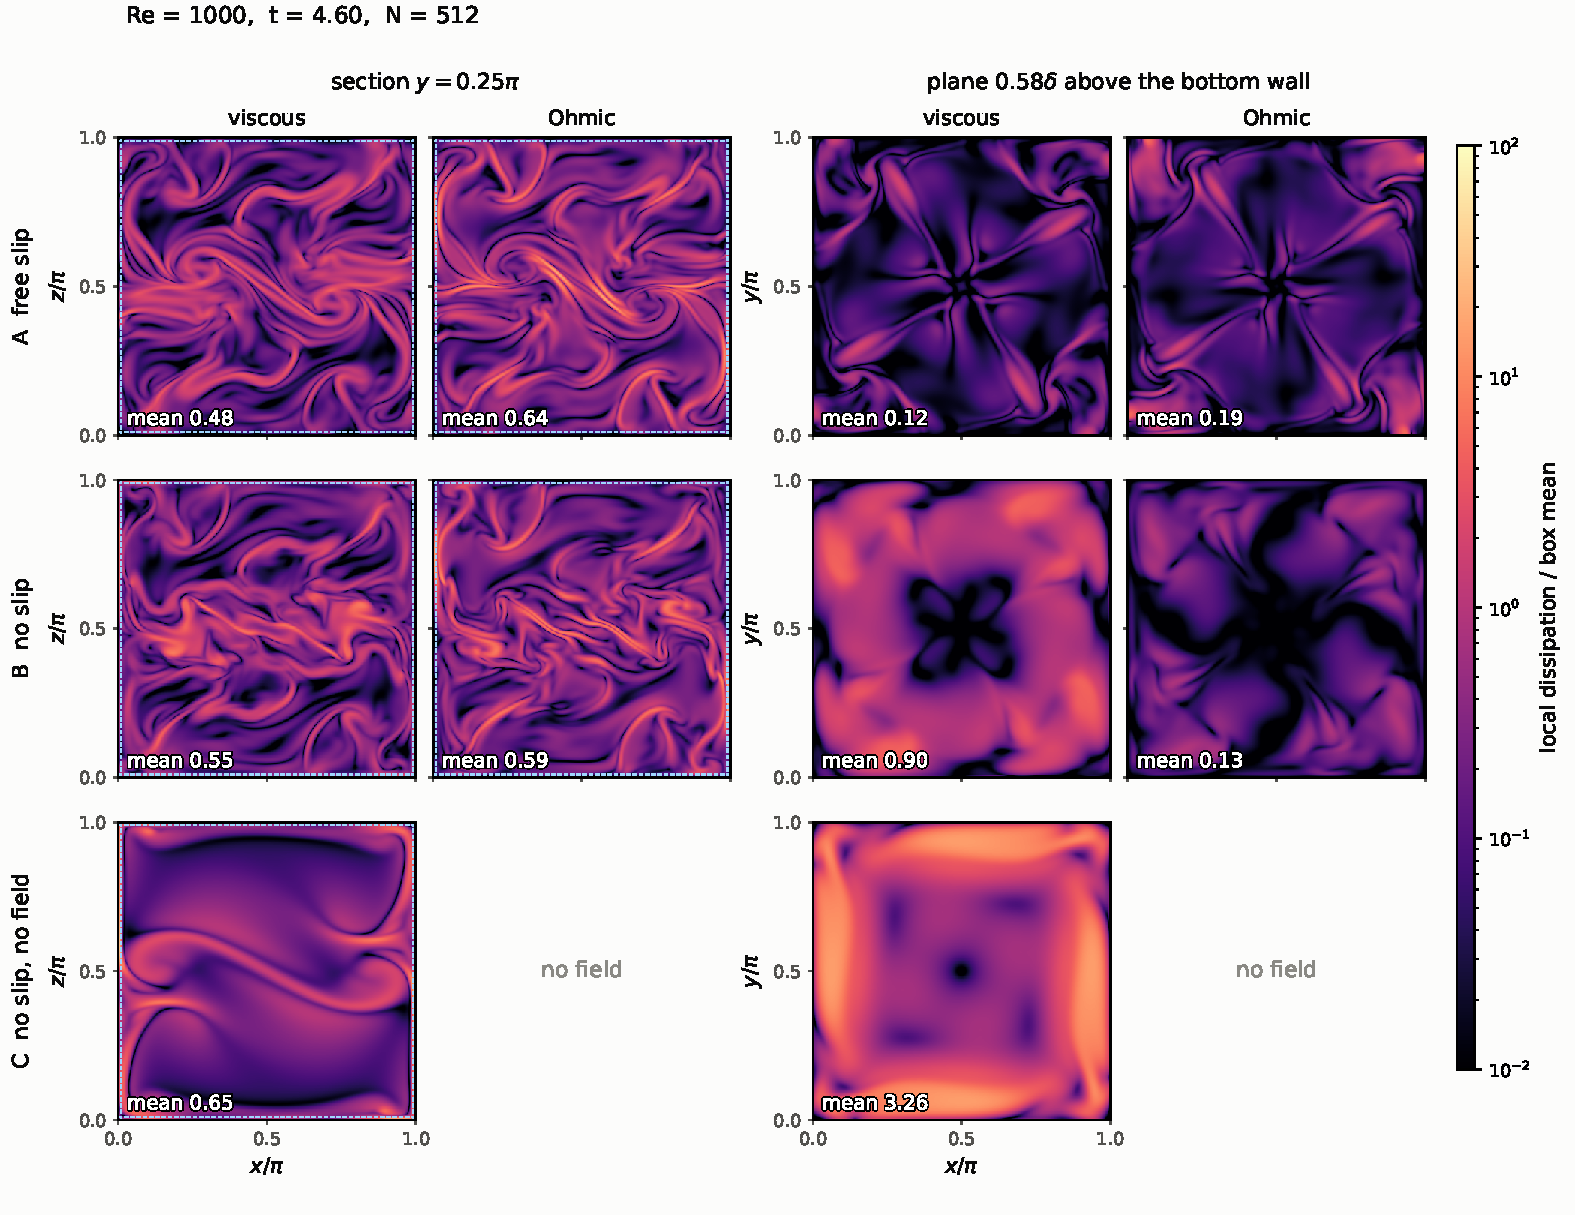
\includegraphics[width=\textwidth]{tg_mhd_snap_t4.6.pdf}
\caption{\label{sfig:snap46}As Fig.~\ref{M-fig:snap23}, at $t=4.6$, by the later
maxima of the dissipation.}
\end{figure*}

\begin{figure*}
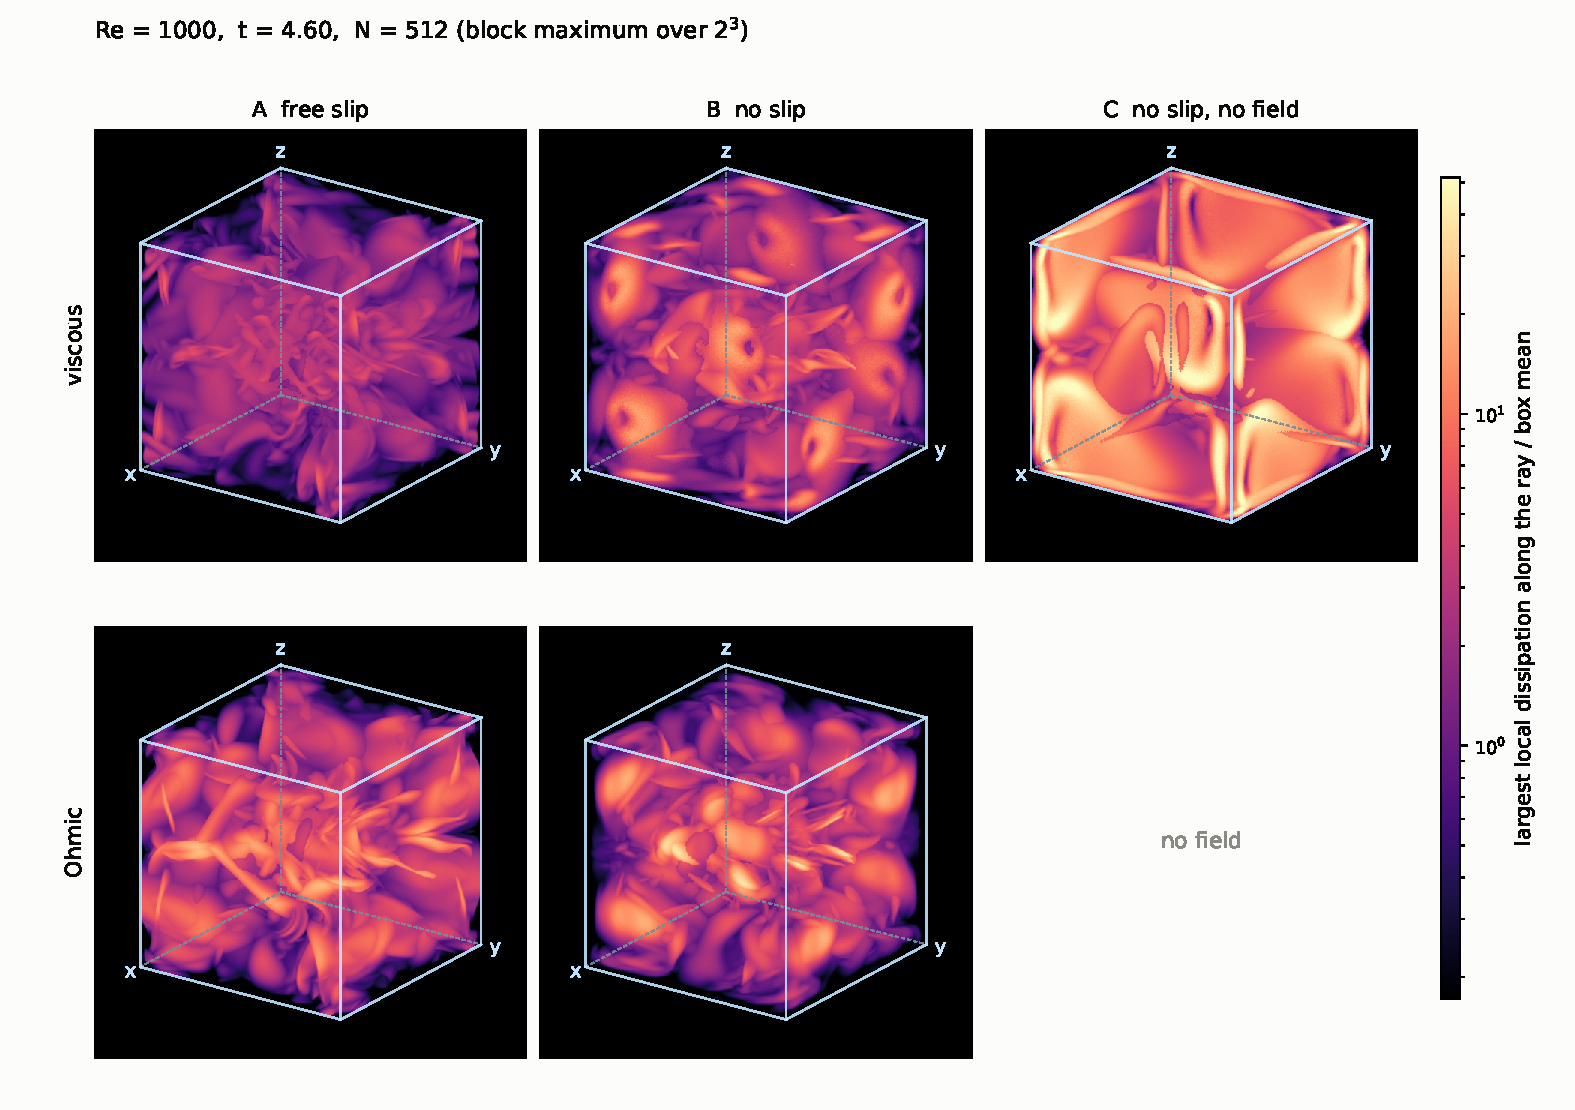
\includegraphics[width=\textwidth]{tg_mhd_3d_t4.6.pdf}
\caption{\label{sfig:vol46}As Fig.~\ref{M-fig:vol23}, at $t=4.6$, on the same colour
scale.}
\end{figure*}

\bibliography{refs}

\end{document}
